% paper/oe_main.tex -- Applied Optics manuscript, media-in-the-loop
% holography (Part 2).
%
% REWRITE 2026-09-26 (PATH_TO_7.md, must-do #1). Written against numbers.tex
% regenerated from the post-freeze results only (n_z = 128, unslanted, complete
% M1 cells only -- analysis/aggregate.py::split_complete_m1). Every number in
% this file is a macro; scripts/check_consistency.py fails the build otherwise.
%
% Evidence classes used throughout (see Section 1 and Supplement S10):
%   [L] literature-reported / established theory -- always cited;
%   [P] a stated HoloForge model or simulation parameter (Table 1, Sec. 3-4);
%   [D] derived here from stated inputs by an equation or algorithm;
%   [S] a simulation output of this study (a "measurement" in the twin).
% Interpretations that go beyond what the data directly show are labelled
% "Interpretation" in the text.
%
% Template: optica-article.cls (Optica Universal Manuscript Template).

\documentclass{optica-article}
\journal{opticajournal}
\articletype{Research Article}
\usepackage{amsmath}
% AUTO-GENERATED by scripts/make_numbers_tex.py -- DO NOT HAND-EDIT.
% Regenerate: python scripts/make_numbers_tex.py
\usepackage{xcolor}  % for the [PENDING] flag color, harmless if already loaded

\newcommand{\MeasuredContrastTwoX}{2.00}
\newcommand{\KcPredTwoX}{4.22}
\newcommand{\KstarTwoXInterp}{4.18}
\newcommand{\KstarTwoXCI}{\textcolor{red}{[PENDING]}}
\newcommand{\MeanGainTwoX}{0.40}
\newcommand{\MinGainTwoX}{-0.03}
\newcommand{\MeasuredContrastFourX}{3.80}
\newcommand{\KcPredFourX}{6.96}
\newcommand{\KstarFourXInterp}{\textcolor{red}{[PENDING]}}
\newcommand{\KstarFourXCI}{8.98}
\newcommand{\MeanGainFourX}{0.70}
\newcommand{\MinGainFourX}{0.04}
\newcommand{\MeasuredContrastEightX}{5.32}
\newcommand{\KcPredEightX}{9.33}
\newcommand{\KstarEightXInterp}{\textcolor{red}{[PENDING]}}
\newcommand{\KstarEightXCI}{8.98}
\newcommand{\MeanGainEightX}{0.88}
\newcommand{\MinGainEightX}{0.05}
\newcommand{\MinGainAllBudgets}{-0.03}
\newcommand{\SEightGainKLowSlantZero}{0.913}
\newcommand{\SEightLoKLowSlantZero}{0.906}
\newcommand{\SEightHiKLowSlantZero}{0.920}
\newcommand{\SEightGainKLowSlantTwoFive}{3.122}
\newcommand{\SEightLoKLowSlantTwoFive}{3.122}
\newcommand{\SEightHiKLowSlantTwoFive}{3.123}
\newcommand{\SEightGainKLowSlantFive}{2.077}
\newcommand{\SEightLoKLowSlantFive}{2.076}
\newcommand{\SEightHiKLowSlantFive}{2.078}
\newcommand{\SEightGainKLowSlantSevenFive}{0.227}
\newcommand{\SEightLoKLowSlantSevenFive}{0.223}
\newcommand{\SEightHiKLowSlantSevenFive}{0.230}
\newcommand{\SEightGainKLowSlantTen}{0.089}
\newcommand{\SEightLoKLowSlantTen}{0.089}
\newcommand{\SEightHiKLowSlantTen}{0.089}
\newcommand{\SEightGainKLowSlantFifteen}{-0.007}
\newcommand{\SEightLoKLowSlantFifteen}{-0.016}
\newcommand{\SEightHiKLowSlantFifteen}{0.002}
\newcommand{\SEightGainKLowSlantTwenty}{0.024}
\newcommand{\SEightLoKLowSlantTwenty}{0.019}
\newcommand{\SEightHiKLowSlantTwenty}{0.028}
\newcommand{\SEightGainKMidSlantZero}{0.899}
\newcommand{\SEightLoKMidSlantZero}{0.898}
\newcommand{\SEightHiKMidSlantZero}{0.901}
\newcommand{\SEightGainKMidSlantTwoFive}{1.017}
\newcommand{\SEightLoKMidSlantTwoFive}{0.980}
\newcommand{\SEightHiKMidSlantTwoFive}{1.055}
\newcommand{\SEightGainKMidSlantFive}{2.045}
\newcommand{\SEightLoKMidSlantFive}{2.044}
\newcommand{\SEightHiKMidSlantFive}{2.046}
\newcommand{\SEightGainKMidSlantSevenFive}{0.291}
\newcommand{\SEightLoKMidSlantSevenFive}{0.210}
\newcommand{\SEightHiKMidSlantSevenFive}{0.371}
\newcommand{\SEightGainKMidSlantTen}{0.185}
\newcommand{\SEightLoKMidSlantTen}{0.182}
\newcommand{\SEightHiKMidSlantTen}{0.187}
\newcommand{\SEightGainKMidSlantFifteen}{0.046}
\newcommand{\SEightLoKMidSlantFifteen}{0.045}
\newcommand{\SEightHiKMidSlantFifteen}{0.046}
\newcommand{\SEightGainKMidSlantTwenty}{0.011}
\newcommand{\SEightLoKMidSlantTwenty}{0.011}
\newcommand{\SEightHiKMidSlantTwenty}{0.011}
\newcommand{\NZZeroPooledGainThirtyTwo}{0.640}
\newcommand{\NZZeroPooledLoThirtyTwo}{0.640}
\newcommand{\NZZeroPooledHiThirtyTwo}{0.640}
\newcommand{\NZZeroPooledGainOneTwentyEight}{0.641}
\newcommand{\NZZeroPooledLoOneTwentyEight}{0.641}
\newcommand{\NZZeroPooledHiOneTwentyEight}{0.641}
\newcommand{\NZZeroPooledGainTwoFiftySix}{0.645}
\newcommand{\NZZeroPooledLoTwoFiftySix}{0.645}
\newcommand{\NZZeroPooledHiTwoFiftySix}{0.645}
\newcommand{\NZZeroGainKLowThirtyTwo}{1.019}
\newcommand{\NZZeroGainKLowOneTwentyEight}{0.915}
\newcommand{\NZZeroGainKLowTwoFiftySix}{0.894}
\newcommand{\NZZeroGainKMidThirtyTwo}{0.731}
\newcommand{\NZZeroGainKMidOneTwentyEight}{0.900}
\newcommand{\NZZeroGainKMidTwoFiftySix}{0.928}
\newcommand{\SOneBaselineGain}{1.81}
\newcommand{\SOneNoSaturationGain}{2.22}
\newcommand{\SOneNoSaturationRatio}{1.2}
\newcommand{\SOneNoDiffusionRatio}{1.14}
\newcommand{\SOneNoNonlocalityRatio}{0.98}
\newcommand{\SOneNoDyeDepletionRatio}{0.98}
\newcommand{\STwoBaselineGain}{0.11}
\newcommand{\STwoGainMin}{0.08}
\newcommand{\STwoGainMax}{0.15}
\newcommand{\SThreeNominalGain}{1.81}
\newcommand{\SThreeWorstWithinFifty}{1.17}
\newcommand{\SThreeWorstWithinFiftyParam}{dn\_max}
\newcommand{\SThreeBestWithinFifty}{1.92}
\newcommand{\SThreeDnMaxFlipPct}{473}
\newcommand{\SThreeDnMaxWorstGain}{-3.73}
\newcommand{\SThreeDnMaxAtHundred}{0.99}
\newcommand{\SThreeDnMaxMostNegativePct}{-83}
\newcommand{\SThreeDnMaxAtMostNegative}{0.38}
\newcommand{\SThreeDnMaxMostPositivePct}{473}
\newcommand{\SThreeDnMaxAtMostPositive}{-3.73}
\newcommand{\SThreeAnyFlipWithinFifty}{no}
\newcommand{\SATMeanGainTwoX}{0.07}
\newcommand{\SATFracOfMILTwoX}{18}
\newcommand{\SATMeanGainFourX}{0.20}
\newcommand{\SATFracOfMILFourX}{28}
\newcommand{\SATMeanGainEightX}{0.36}
\newcommand{\SATFracOfMILEightX}{42}
\newcommand{\SATFitNRMSE}{0.103}
\newcommand{\SATFitAEff}{7.05}
\newcommand{\SATSubCliffGain}{0.98}
\newcommand{\SATSubCliffMILGain}{1.37}
\newcommand{\SATSubCliffFracOfMIL}{71}
\newcommand{\SATSubCliffFracMin}{79}
\newcommand{\SATSubCliffFracMax}{79}
\newcommand{\SATSubCliffK}{1.31}
\newcommand{\SATNearCliffK}{3.93}
\newcommand{\SATNearCliffFrac}{56}
\newcommand{\SATPostCliffK}{5.24}
\newcommand{\SATPostCliffFracMin}{-28}
\newcommand{\SATPostCliffFracMax}{-28}
\newcommand{\SeedCountMin}{3}
\newcommand{\SeedCountMax}{3}
\newcommand{\SeedCountDesc}{3}
\newcommand{\SeedCountModal}{3}
\newcommand{\SeedCountNExtraConfigs}{0}
\newcommand{\SeedCount}{3}
\newcommand{\NResultFiles}{2375}

% --- supplement macros (already-real data, not Phase-3-gated) ---
\newcommand{\AblationCheckpointCosSim}{1.000}
\newcommand{\AblationSurrogateCosSim}{0.844}
\newcommand{\RCWAMaxDevThreeCase}{0.038}
\newcommand{\RCWAVGridMaxDev}{0.980}
\newcommand{\RCWAVGridNCases}{90}
\newcommand{\RCWAUnslantedMaxDev}{0.29}
\newcommand{\RCWANormalMedianDev}{0.001}
\newcommand{\MeshPSNRSpread}{0.036}
\newcommand{\WavelengthDesignPSNR}{6.63}

% --- validation (Phase 6 / Section 6) macros ---
\newcommand{\NLiteratureSources}{3}
\newcommand{\NRMSEBruderGrowthDnKExp}{0.28}
\newcommand{\NRMSEBruderGrowthDnKSim}{0.17}
\newcommand{\NRMSEHsiehGrowthDnK}{0.10}
\newcommand{\NRMSEWorstFit}{0.28}
\newcommand{\NRMSEBestFit}{0.10}
\newcommand{\NGoodFits}{3}
\newcommand{\NRMSEWorstInRegime}{0.28}
\newcommand{\NRMSEBestInRegime}{0.17}
\newcommand{\NInRegimeSources}{2}
\newcommand{\BayfolDnMaxRatio}{5.7}

% --- baseline completeness (Sec. 5.2 / F4b) macros ---
\newcommand{\GSGainMin}{-1.27}
\newcommand{\GSGainMax}{0.00}
\newcommand{\LPCGainMin}{-1.82}
\newcommand{\LPCGainMax}{0.07}
\newcommand{\MILGainMinAtTwoX}{-0.03}

% --- shrinkage-induced shift bound (Discussion) macros ---
\newcommand{\ShrinkagePct}{0.5}
\newcommand{\ShrinkageSlantDeg}{20}
\newcommand{\ShrinkageThicknessUm}{30}
\newcommand{\ShrinkageShiftNm}{54.6}
\newcommand{\ShrinkageFracLowK}{1.7}
\newcommand{\ShrinkageFracHighK}{13.7}

% --- cost-benefit (Sec. 5.1) macros ---
\newcommand{\ComputeMatchRatio}{21.7}

% --- R1 reconstruction figure macros ---
\newcommand{\ROneSeedValue}{0}

% --- WP3 baseline (RSGD/GPC, Sec. 5.2) macros ---
\newcommand{\RSGDGainMin}{-0.00}
\newcommand{\RSGDGainMax}{0.00}
\newcommand{\GPCGainMin}{-1.98}
\newcommand{\GPCGainMax}{0.07}
\newcommand{\GPCLPCMaxAbsDiffTwoX}{0.18}

% --- WP4 (target ensemble / noise robustness, Sec. 5.x) macros ---
\newcommand{\SFourGainBarsTwoX}{0.90}
\newcommand{\SFourBootCILoBarsTwoX}{0.90}
\newcommand{\SFourBootCIHiBarsTwoX}{0.90}
\newcommand{\SFourGainBarsEightX}{1.95}
\newcommand{\SFourBootCILoBarsEightX}{1.95}
\newcommand{\SFourBootCIHiBarsEightX}{1.95}
\newcommand{\SFourGainSpotsTwoX}{3.22}
\newcommand{\SFourBootCILoSpotsTwoX}{3.19}
\newcommand{\SFourBootCIHiSpotsTwoX}{3.23}
\newcommand{\SFourGainSpotsEightX}{4.07}
\newcommand{\SFourBootCILoSpotsEightX}{3.99}
\newcommand{\SFourBootCIHiSpotsEightX}{4.12}
\newcommand{\SFourGainRandomBinaryTwoX}{0.17}
\newcommand{\SFourBootCILoRandomBinaryTwoX}{0.17}
\newcommand{\SFourBootCIHiRandomBinaryTwoX}{0.17}
\newcommand{\SFourGainRandomBinaryEightX}{0.24}
\newcommand{\SFourBootCILoRandomBinaryEightX}{0.24}
\newcommand{\SFourBootCIHiRandomBinaryEightX}{0.24}
\newcommand{\SFiveNoiseStdPct}{5}
\newcommand{\SFiveNoiselessGain}{0.90}
\newcommand{\SFiveNoisyGain}{0.88}

% --- WP5 (joint miscalibration Monte Carlo, Sec. 5.x) macros ---
\newcommand{\SSixNDraws}{30}
\newcommand{\SSixMeanGain}{1.76}
\newcommand{\SSixBootCILo}{1.73}
\newcommand{\SSixBootCIHi}{1.79}
\newcommand{\SSixNNegative}{0}
\newcommand{\SSixWorstDrawGain}{1.61}
\newcommand{\SSixBestDrawGain}{1.94}
\newcommand{\SSixPctRange}{25}

% --- WP6 (depth-resolved absorption, Sec. 5.x) macros ---
\newcommand{\SSevenGainODZero}{1.81}
\newcommand{\SSevenGainODOneTenth}{1.51}
\newcommand{\SSevenGainODThreeTenths}{1.45}

% --- PATH_TO_7 rewrite macros (complete M1 cells only) ---
\newcommand{\MOneNK}{10}
\newcommand{\MOneNCells}{30}
\newcommand{\MOneKMin}{1.96}
\newcommand{\MOneKMax}{15.71}
\newcommand{\MOneKList}{1.96, 2.62, 3.49, 3.93, 4.19, 4.83, 5.71, 6.98, 8.98, 15.71}
\newcommand{\MOneNPositive}{29}
\newcommand{\MOneNCIAboveZero}{27}
\newcommand{\MOneNCIIncludesZero}{2}
\newcommand{\MOneNNegative}{1}
\newcommand{\MOneNegK}{4.19}
\newcommand{\MOneNegBudget}{2}
\newcommand{\MOneNegGain}{-0.03}
\newcommand{\MOneNegCILo}{-0.05}
\newcommand{\MOneNegCIHi}{-0.005}
\newcommand{\MaxGainTwoX}{1.42}
\newcommand{\MaxGainKTwoX}{2.62}
\newcommand{\GainHighKTwoX}{0.01}
\newcommand{\GainHighKLoTwoX}{0.002}
\newcommand{\GainHighKHiTwoX}{0.008}
\newcommand{\MaxGainFourX}{2.13}
\newcommand{\MaxGainKFourX}{1.96}
\newcommand{\GainHighKFourX}{0.04}
\newcommand{\GainHighKLoFourX}{0.009}
\newcommand{\GainHighKHiFourX}{0.062}
\newcommand{\MaxGainEightX}{2.52}
\newcommand{\MaxGainKEightX}{2.62}
\newcommand{\GainHighKEightX}{0.05}
\newcommand{\GainHighKLoEightX}{0.019}
\newcommand{\GainHighKHiEightX}{0.091}
\newcommand{\MOneNExcluded}{0}
\newcommand{\SOneGBaselineSub}{4.41}
\newcommand{\SOneGBaselineNear}{0.90}
\newcommand{\SOneGBaselinePost}{0.11}
\newcommand{\SOneGNoSatSub}{5.39}
\newcommand{\SOneGNoSatNear}{0.61}
\newcommand{\SOneGNoSatPost}{0.66}
\newcommand{\SOneGNoDiffSub}{4.93}
\newcommand{\SOneGNoDiffNear}{1.14}
\newcommand{\SOneGNoDiffPost}{0.10}
\newcommand{\SOneGNoNonlocSub}{4.47}
\newcommand{\SOneGNoNonlocNear}{0.82}
\newcommand{\SOneGNoNonlocPost}{0.05}
\newcommand{\SOneGNoDyeSub}{4.36}
\newcommand{\SOneGNoDyeNear}{0.84}
\newcommand{\SOneGNoDyePost}{0.11}
\newcommand{\SOneKSub}{1.31}
\newcommand{\SOneKNear}{3.93}
\newcommand{\SOneKPost}{5.24}
\newcommand{\SXGBaselineSub}{4.41}
\newcommand{\SXNBaselineSub}{3}
\newcommand{\SXGBaselineNear}{0.90}
\newcommand{\SXNBaselineNear}{3}
\newcommand{\SXGBaselinePost}{0.11}
\newcommand{\SXNBaselinePost}{3}
\newcommand{\SXGNoMonomerSub}{-0.12}
\newcommand{\SXNNoMonomerSub}{3}
\newcommand{\SXGNoMonomerNear}{-0.09}
\newcommand{\SXNNoMonomerNear}{3}
\newcommand{\SXGNoMonomerPost}{-0.08}
\newcommand{\SXNNoMonomerPost}{3}
\newcommand{\SXGNoDyeSub}{4.35}
\newcommand{\SXNNoDyeSub}{3}
\newcommand{\SXGNoDyeNear}{0.84}
\newcommand{\SXNNoDyeNear}{3}
\newcommand{\SXGNoDyePost}{0.11}
\newcommand{\SXNNoDyePost}{3}
\newcommand{\SXGNoSatSub}{5.38}
\newcommand{\SXNNoSatSub}{3}
\newcommand{\SXGNoSatNear}{0.62}
\newcommand{\SXNNoSatNear}{3}
\newcommand{\SXGNoSatPost}{0.66}
\newcommand{\SXNNoSatPost}{3}
\newcommand{\SXGOnlyTanhSub}{-0.10}
\newcommand{\SXNOnlyTanhSub}{3}
\newcommand{\SXGOnlyTanhNear}{-0.02}
\newcommand{\SXNOnlyTanhNear}{3}
\newcommand{\SXGOnlyTanhPost}{-0.03}
\newcommand{\SXNOnlyTanhPost}{3}
\newcommand{\SXGOnlyDyeSub}{14.37}
\newcommand{\SXNOnlyDyeSub}{3}
\newcommand{\SXGOnlyDyeNear}{6.38}
\newcommand{\SXNOnlyDyeNear}{3}
\newcommand{\SXGOnlyDyePost}{7.40}
\newcommand{\SXNOnlyDyePost}{3}
\newcommand{\SXGOnlyMonomerSub}{5.75}
\newcommand{\SXNOnlyMonomerSub}{3}
\newcommand{\SXGOnlyMonomerNear}{1.73}
\newcommand{\SXNOnlyMonomerNear}{3}
\newcommand{\SXGOnlyMonomerPost}{1.26}
\newcommand{\SXNOnlyMonomerPost}{3}
\newcommand{\SXGLinearSub}{14.94}
\newcommand{\SXNLinearSub}{3}
\newcommand{\SXGLinearNear}{7.66}
\newcommand{\SXNLinearNear}{3}
\newcommand{\SXGLinearPost}{9.04}
\newcommand{\SXNLinearPost}{3}
\newcommand{\SXGLinearMatchedSub}{-0.00}
\newcommand{\SXNLinearMatchedSub}{3}
\newcommand{\SXGLinearMatchedNear}{0.00}
\newcommand{\SXNLinearMatchedNear}{3}
\newcommand{\SXGLinearMatchedPost}{0.10}
\newcommand{\SXNLinearMatchedPost}{3}
\newcommand{\SXGNoMonomerMatchedSub}{3.64}
\newcommand{\SXNNoMonomerMatchedSub}{3}
\newcommand{\SXGNoMonomerMatchedNear}{0.72}
\newcommand{\SXNNoMonomerMatchedNear}{3}
\newcommand{\SXGNoMonomerMatchedPost}{0.08}
\newcommand{\SXNNoMonomerMatchedPost}{3}
\newcommand{\SXGOnlyDyeMatchedSub}{1.98}
\newcommand{\SXNOnlyDyeMatchedSub}{3}
\newcommand{\SXGOnlyDyeMatchedNear}{0.42}
\newcommand{\SXNOnlyDyeMatchedNear}{3}
\newcommand{\SXGOnlyDyeMatchedPost}{-0.02}
\newcommand{\SXNOnlyDyeMatchedPost}{3}
\newcommand{\SXGOnlyTanhMatchedSub}{2.80}
\newcommand{\SXNOnlyTanhMatchedSub}{3}
\newcommand{\SXGOnlyTanhMatchedNear}{0.53}
\newcommand{\SXNOnlyTanhMatchedNear}{3}
\newcommand{\SXGOnlyTanhMatchedPost}{0.12}
\newcommand{\SXNOnlyTanhMatchedPost}{3}
\newcommand{\SXDeviceMaxDiff}{0.001}
\newcommand{\SATFracLowKMin}{36}
\newcommand{\SATFracLowKMax}{44}
\newcommand{\SATFracSecondKMin}{53}
\newcommand{\SATFracSecondKMax}{66}
\newcommand{\SATNBelowBSGD}{12}
\newcommand{\SATNCells}{29}
\newcommand{\SThreeDnMaxAtMinusFifty}{1.17}
\newcommand{\SThreeDnMaxAtPlusFifty}{1.66}
\newcommand{\MTwoRGainSub}{3.19}
\newcommand{\MTwoRLoSub}{2.94}
\newcommand{\MTwoRHiSub}{3.43}
\newcommand{\MTwoRGainNear}{0.81}
\newcommand{\MTwoRLoNear}{0.81}
\newcommand{\MTwoRHiNear}{0.81}
\newcommand{\MTwoRGainPost}{0.12}
\newcommand{\MTwoRLoPost}{0.12}
\newcommand{\MTwoRHiPost}{0.13}
\newcommand{\MTwoRSATFracSub}{79}
\newcommand{\MTwoRSATFracNear}{56}
\newcommand{\MTwoRSATFracPost}{-28}
\newcommand{\HoldoutASimIn}{0.17}
\newcommand{\HoldoutASimOut}{0.48}
\newcommand{\HoldoutASimKbleach}{\textcolor{red}{[PENDING]}}
\newcommand{\HoldoutASimDnMax}{0.0504}
\newcommand{\HoldoutASimAtBound}{none}
\newcommand{\HoldoutAExpIn}{0.28}
\newcommand{\HoldoutAExpOut}{1.09}
\newcommand{\HoldoutAExpKbleach}{\textcolor{red}{[PENDING]}}
\newcommand{\HoldoutAExpDnMax}{0.289}
\newcommand{\HoldoutAExpAtBound}{none}
\newcommand{\HoldoutBSimIn}{0.02}
\newcommand{\HoldoutBSimOut}{0.40}
\newcommand{\HoldoutBSimKbleach}{0.0667}
\newcommand{\HoldoutBSimDnMax}{0.0418}
\newcommand{\HoldoutBSimAtBound}{none}
\newcommand{\HoldoutBExpIn}{0.17}
\newcommand{\HoldoutBExpOut}{0.31}
\newcommand{\HoldoutBExpKbleach}{0.0215}
\newcommand{\HoldoutBExpDnMax}{0.0321}
\newcommand{\HoldoutBExpAtBound}{none}

% --- diffraction-efficiency confirmation (Sec. 5.1) macros ---
\newcommand{\DEMeanGainTwoX}{1.80}
\newcommand{\DEMeanGainFourX}{3.00}
\newcommand{\DEMeanGainEightX}{3.94}
\newcommand{\DEMinGainAllBudgets}{-0.251}
\newcommand{\DENNegative}{15}
\newcommand{\DENPairs}{90}

% --- wasted-media measurement (Sec. 5.4) macros ---
\newcommand{\WastedMediaThreshDB}{2}
\newcommand{\WastedMediaBSGDFrac}{37}
\newcommand{\WastedMediaMILFrac}{0}
\newcommand{\WastedMediaBSGDFracOneDB}{60}
\newcommand{\WastedMediaMILFracOneDB}{57}
\newcommand{\WastedMediaBSGDFracThreeDB}{17}
\newcommand{\WastedMediaMILFracThreeDB}{0}
\newcommand{\WastedMediaNConfigs}{30}
\newcommand{\WastedMediaGSFrac}{53}
\newcommand{\WastedMediaGSFracOneDB}{60}
\newcommand{\WastedMediaGSFracThreeDB}{33}
\newcommand{\WastedMediaLPCFrac}{47}
\newcommand{\WastedMediaLPCFracOneDB}{60}
\newcommand{\WastedMediaLPCFracThreeDB}{33}
\newcommand{\WastedMediaSATFrac}{33}
\newcommand{\WastedMediaSATFracOneDB}{60}
\newcommand{\WastedMediaSATFracThreeDB}{0}
\newcommand{\WastedMediaRSGDFrac}{37}
\newcommand{\WastedMediaRSGDFracOneDB}{60}
\newcommand{\WastedMediaRSGDFracThreeDB}{17}
\newcommand{\WastedMediaGPCFrac}{47}
\newcommand{\WastedMediaGPCFracOneDB}{60}
\newcommand{\WastedMediaGPCFracThreeDB}{30}
  % scripts/make_numbers_tex.py output -- all quantitative macros

\begin{document}

\title{Media-in-the-Loop Holography: Computer-Generated Holography\\
Through a Differentiable Model of Volume Photopolymer Recording}

\author{Chaitanya Tripathi\authormark{1,*}}

\address{\authormark{1}Ashoka University, Sonipat, India}

\email{\authormark{*}chaitanya.tripathi\_ug2025@ashoka.edu.in}

\begin{abstract*}
Camera-in-the-loop correction is unavailable for write-once volume
photopolymers, because the reconstruction error can be measured only after
it is permanent. We study, in simulation, the alternative of placing a
differentiable model of the recording chemistry -- a non-local
polymerization-driven diffusion (NPDD) model coupled to split-step
beam-propagation readout -- inside the exposure-design loop. On an
unslanted one-dimensional grating benchmark of \MOneNCells{}
spatial-frequency/contrast-budget cells, the simulated gain over a
media-blind optimizer is positive in \MOneNPositive{} cells (at most
\MaxGainEightX{}\,dB) and decays toward zero at high spatial frequency. The
fraction of exposures more than \WastedMediaThreshDB\,dB short of an oracle
reference falls from \WastedMediaBSGDFrac\% to \WastedMediaMILFrac\%; at a
1\,dB threshold the two methods are similar. The gain largely disappears
for fringes slanted by $10^\circ$ or more. The twin is checked against one
published photopolymer family only; all results are simulation outputs,
reproducible from the released code.
\end{abstract*}

% ======================================================================
\section{Introduction}
Phase-only computer-generated holography (CGH) computes a modulation
pattern whose diffracted field approximates a target. Camera-in-the-loop
(CITL) optimization reduces the mismatch between a computed pattern and a
physical spatial light modulator by measuring the reconstruction and
back-propagating the residual into the display model~\cite{peng2020neural}.
That feedback loop requires a rewritable modulator.

Volume photopolymers -- Bayfol HX~\cite{bruder2017bayfol},
acrylamide/PVA, PQ/PMMA~\cite{hsieh2022pqpmma} -- record a permanent
refractive-index distribution formed by photopolymerization and mass
transport. The recorded index profile is not a scaled copy of the exposure:
monomer diffusion~\cite{zhao1994diffusion,sheridan2012reply}, non-local
chain growth~\cite{sheridan2000nonlocal,gleeson2008chain}, dye depletion
and a saturating index response each act nonlinearly on the exposure
[L]. Because the medium is write-once, a CITL-style measurement of the
reconstruction error arrives only after the error has become permanent.

This paper asks, entirely in simulation, how much an exposure optimized
through a differentiable model of the recording process (``media-in-the-loop'',
MIL) improves on the same optimizer run with a linear, media-blind recording
assumption, and where that improvement comes from. The contribution is an
engineering synthesis and a characterization, not a new physical model: the
recording model (NPDD), the readout model (split-step beam propagation) and
the optimizer (Adam with reverse-mode automatic differentiation) are
established and cited where they are introduced; what is ours is their
combination into an exposure-domain design loop and the systematic
simulated evaluation of that loop (Section~\ref{sec:results}).

\textbf{How claims are sourced.} Every quantitative statement belongs to one
of four classes, marked where the distinction matters: literature-reported
or established theory [L], always cited; a stated HoloForge model or
simulation parameter [P] (Table~\ref{tab:mediumparams}, Sections~\ref{sec:model}--\ref{sec:method}); a result derived here by an equation or
algorithm from stated inputs [D]; and a simulation output of this study
[S]. [S] results are measurements \emph{in the twin}, not of a physical
medium, and are reported with the seed count and interval method used.
Statements that go beyond what the data directly show are labelled as
interpretation. Supplement S10 maps each headline number to its source
file and generating script.

\textbf{Why a paired design, and what it does not buy.} Every headline
number is a paired difference -- MIL minus media-blind SGD -- with both arms
designed and scored against the same twin instance. An
exposure-independent calibration error in the twin (an offset or a ceiling
error common to every exposure) cancels in that difference [D]. An
exposure-dependent twin-vs-reality gap does not cancel, because the two arms
record different exposures. We therefore also test one-sided robustness
directly: the exposure is designed on the nominal twin and scored on a
deliberately miscalibrated one (Section~\ref{sec:mismatch}).

This work is the second of a two-part study; Part~1 characterized phase-only
CGH degradation under idealized-modulator assumptions~\cite{tripathi2025holoforge}.

% ======================================================================
\section{Related work}
\textbf{Model-mismatch correction for holographic displays.}
CITL~\cite{peng2020neural}, Wirtinger holography~\cite{chakravarthula2019wirtinger},
learned proxy models~\cite{shi2021towards} and time-multiplexed control of
quantized modulators~\cite{choi2022time} correct a display model with
camera measurements of a rewritable modulator. In the write-once setting
considered here the model has to carry that burden without feedback.

\textbf{Fabrication-aware design.} Neural lithography~\cite{zheng2023neural}
places a learned twin of a lithographic process inside differentiable
design of surface-relief optics. Adjoint inverse design~\cite{hughes2018adjoint}
treats a physical forward model as a differentiable layer; MIL applies the
same pattern to a recording chemistry's governing PDE. Proximity-effect
correction in electron-beam lithography~\cite{li2015proximity} is a
correction problem bounded by the resist's response, conceptually related
though physically unrelated.

\textbf{Concurrent work.} Wechsler et al.~\cite{wechsler2026shvam} couple a
differentiable wave-optical model to a photochemical model for holographic
volumetric printing, with inhibitor diffusion but no non-local production
kernel, and demonstrate printed parts experimentally -- evidence this
simulation study does not provide. The present work addresses a
Bragg-selective index grating scored by diffraction, and contributes a
simulated characterization across spatial frequency, contrast budget,
recording mechanism, grating slant and twin miscalibration. We make no
priority claim for differentiable recording models in a design loop.

% ======================================================================
\section{Model}
\label{sec:model}
Sections~\ref{sec:model-exposure}--\ref{sec:model-loss} specify the forward
model completely; Table~\ref{tab:mediumparams} lists every physical
constant and its source class. The released code is the reference
implementation.

\subsection{Exposure and feasible set [P]}
\label{sec:model-exposure}
The design variable is the delivered exposure $E(x)\ge 0$ on the transverse
coordinate $x$, constrained to a mean dose $E_0$ and a peak-to-mean
contrast budget $B_c$:
\begin{equation}
\label{eq:feasible-set}
\mathcal{E}(E_0,B_c)=\Big\{E:\;E\ge0,\;\overline{E}=E_0,\;
\max_x E(x)/\overline{E}\le B_c\Big\}.
\end{equation}
After every optimizer step the exposure is projected onto $\mathcal{E}$ by
20 alternating passes of dose rescaling $E\leftarrow E\,E_0/(\overline{E}+\epsilon)$
and peak clipping $E\leftarrow\min(E,B_cE_0)$ [P]. Both operations are
elementwise and differentiable. The residual constraint violation after
20 passes is below $10^{-6}$ (relative) on the tested targets [S].

\subsection{Recording: NPDD [L] with stated simplifications [P]}
\label{sec:model-npdd}
Free monomer $u(x,t)$ ($u(x,0)=1$), polymer $N(x,t)$ ($N(x,0)=0$) and
unreacted dye $d(x,t)$ ($d(x,0)=1$) evolve as in the non-local
polymerization-driven diffusion model~\cite{sheridan2000nonlocal}, itself
built on the local model of Zhao and Mouroulis~\cite{zhao1994diffusion}:
\begin{align}
\partial_t u &= \partial_x\!\big(D_{\text{eff}}(N)\,\partial_x u\big) - G_\sigma*(F u), \label{eq:npdd-u}\\
\partial_t N &= G_\sigma*(F u), \label{eq:npdd-N}\\
\partial_t d &= -k_{\text{bleach}}\,I\,d, \label{eq:npdd-d}
\end{align}
with $F=\kappa\,(I d)^\gamma$, a Gaussian non-local kernel
$G_\sigma$ of width $\sigma$ ($\widehat{G_\sigma}(K)=e^{-K^2\sigma^2/2}$),
and $D_{\text{eff}}(N)=D_0e^{-\alpha_D N}$. The kernel acts on the production
term $Fu$: polymer initiated at $x'$ is deposited at $x$~\cite{sheridan2000nonlocal}.
The recorded index modulation is
\begin{equation}
\label{eq:npdd-dn}
\Delta n(x)=\Delta n_{\max}\tanh\!\big(\beta N(x)\big),\qquad \beta=1.5 .
\end{equation}
The saturating map and the value $\beta=1.5$ are modelling choices of this
work [P], not literature-sourced; every fit in this paper holds $\beta$
fixed. Three mechanisms in this model saturate the dose response: monomer
depletion ($u\to0$), dye bleaching ($d\to0$) and the $\tanh$ map
(Section~\ref{sec:mechanism} separates them).

\subsection{Integrator and gradients [D]}
\label{sec:model-imex}
Equations~\eqref{eq:npdd-u}--\eqref{eq:npdd-d} are integrated over
$t_{\text{total}}=10$\,s in $n_{\text{steps}}=300$ first-order
implicit--explicit steps [P]. The explicit reaction step evaluates the
non-local production by FFT, caps the consumed monomer at the monomer
available (so that $u\ge0$ and $u+N$ is conserved to rounding error), and
updates $d$ exactly for fixed $I$. The implicit diffusion step applies
$\exp(-\bar{D}K^2\,\mathrm{d}t)$ in Fourier space, with $\bar{D}$ the
spatial mean of $D_{\text{eff}}$ -- an approximation to the variable-coefficient
operator in Eq.~\eqref{eq:npdd-u}, whose one-step error we measured as
$\approx0.1\%$ of $u$'s scale at a representative late-trajectory state
[S]; the error accumulated over a full trajectory was not bounded.
Gradients with respect to $E$ are the discrete adjoint of this integrator,
obtained by reverse-mode automatic differentiation through all
$n_{\text{steps}}$~\cite{griewank2008evaluating,paszke2019pytorch}. A
checkpointed variant gives gradients with cosine similarity
\AblationCheckpointCosSim{} to the unrolled ones [S].

\subsection{Readout: split-step beam propagation [L]}
\label{sec:model-readout}
The recorded profile $\Delta n(x)$ is extruded uniformly through a slab of
thickness $T$ [P] and read out at wavelength $\lambda$ by scalar split-step
beam propagation~\cite{feit1978light}: $n_z=128$ slices [P], each applying
the phase $\exp(ik_0\Delta n\,\mathrm{d}z(1-s))$ ($k_0=2\pi/\lambda$,
shrinkage $s$) followed by band-limited angular-spectrum
propagation~\cite{goodman2005fourier}, then one angular-spectrum step to
the reconstruction plane; the reconstruction is the intensity $|E|^2$.
Slanted fringes ($x-z\tan\phi=\text{const}$) are represented by a
per-slice lateral Fourier shift. All headline results use an unslanted
grating ($\phi=0$) [P], the geometry in which this scalar readout agrees
with rigorous coupled-wave analysis (RCWA)~\cite{moharam1981rigorous}
(Section~\ref{sec:discussion}); slant is studied separately
(Section~\ref{sec:slant}). The slice count was checked for convergence at
this geometry: between $n_z=128$ and $256$ the paired gain changes by
\NZZeroGainKLowOneTwentyEight$\to$\NZZeroGainKLowTwoFiftySix\,dB at
$K=1.96$ and \NZZeroGainKMidOneTwentyEight$\to$\NZZeroGainKMidTwoFiftySix\,dB
at $K=3.93$\,rad/\textmu m (one seed; Supplement S3) [S].

\textbf{Diffraction regime [D].} The Klein--Cook parameter
$Q=2\pi\lambda T/(n_0\Lambda^2)$, $\Lambda=2\pi/K$~\cite{klein1967unified},
crosses 10 at $K\approx2.79$\,rad/\textmu m for the default medium, so the
two lowest tested $K$ lie in the intermediate regime rather than the Bragg
regime. Kogelnik coupled-wave theory~\cite{kogelnik1969coupled} is used only
as a closed-form cross-check, never inside an optimization loop.

\subsection{Loss and optimizer [L]+[P]}
\label{sec:model-loss}
With reconstruction $R$ and target intensity $I_t$, the loss is the
scale-invariant mean-squared error
\begin{equation}
\label{eq:si-mse}
\mathcal{L}(R,I_t)=\frac{1}{n_x}\big\|\alpha^\star R-I_t\big\|_2^2\big/\max(I_t)^2,\qquad
\alpha^\star=\langle R,I_t\rangle/\langle R,R\rangle,
\end{equation}
and we report $\mathrm{PSNR}_{\text{si}}=-10\log_{10}\mathcal{L}$, so the
reported metric is a monotone transform of the optimized objective. The
optimizer is Adam~\cite{kingma2015adam} (learning rate $5\times10^{-2}$,
$800$ iterations, convergence tolerance $10^{-4}$) on a softplus
parameterization $E=\mathrm{softplus}(\theta)+10^{-6}$ [P]. The random seed
enters only through the initialization $\theta_0=10^{-2}z$,
$z\sim\mathcal{N}(0,I)$; seed-to-seed spread therefore measures sensitivity
to the starting point, not model or parameter uncertainty.

\begin{table}[htbp]
\centering
\caption{Default medium [P] and the source class of each value. The defaults
are acrylamide/PVA-like illustrative values chosen inside cited ranges;
they are not a refit of one published medium.}
\label{tab:mediumparams}
\begin{tabularx}{\linewidth}{l l X}
\hline
Parameter & Default & Source \\
\hline
$D_0$ & $0.1\,\mu\mathrm{m}^2/\mathrm{s}$ & [P] illustrative; literature value for AA/PVA $0.01$~\cite{sheridan2012reply} [L] \\
$\sigma$ & $0.08\,\mu\mathrm{m}$ & [P] illustrative; literature range $0.01$--$0.04\,\mu\mathrm{m}$~\cite{gleeson2008chain} [L] \\
$\kappa$ & $2.0$ & [P] calibration choice, not literature-read \\
$\gamma$ & $1.0$ & [P] within the literature range $0.5$--$1.0$~\cite{sheridan2000nonlocal} \\
$\Delta n_{\max}$ & $3.5\times10^{-3}$ & [P] within the literature range $1.5$--$5\times10^{-3}$ (AA/PVA) \\
$k_{\text{bleach}}$ & $0.2$ & [P] order of magnitude, not independently sourced \\
$\alpha_D$ & $1.0$ & [P] order of magnitude, not independently sourced \\
$\beta$ & $1.5$ & [P] shape constant of Eq.~\eqref{eq:npdd-dn} \\
$s$ & $0.5\%$ & [P] placeholder of typical AA/PVA magnitude \\
$T$, $n_0$, $\lambda$ & $30\,\mu$m, $1.5$, $405$\,nm & [P] operating point \\
$\phi$ & $0^\circ$ & [P] unslanted; slant swept in Section~\ref{sec:slant} \\
Grid & $n_x=1024$, $\mathrm{d}x=0.05\,\mu$m & [P] $51.2\,\mu$m periodic window \\
\hline
\end{tabularx}
\end{table}

% ======================================================================
\section{Methods compared}
\label{sec:method}
All methods share the exposure parameterization, the projection onto
$\mathcal{E}$ and the scoring on the full twin. \textbf{MIL} optimizes
Eq.~\eqref{eq:si-mse} with the twin (NPDD + BPM) inside the loss.
\textbf{Media-blind SGD (BSGD)} runs the same optimizer with the linear
recording assumption $\Delta n=\Delta n_{\max}(E-\overline{E})$ and no
shrinkage, then scores its exposure on the twin -- the practice MIL is
compared against. \textbf{Gerchberg--Saxton (GS)} is the established
alternating-projection phase-retrieval algorithm~\cite{gerchberg1972practical,fienup1982phase}
[L]; its retrieved phase is converted to an exposure by the same linear
assumption. \textbf{Linear pre-compensation (LPC)} [D] boosts each
spatial-frequency component of the target by $1/H(K)$, with $H(K)$ the
heuristic small-signal transfer function of Supplement S1, then projects.
\textbf{Gamma pre-compensation (GPC)} [D] inverts a fitted pointwise
saturating map in real space. \textbf{TV-regularized SGD (RSGD)} is BSGD
with a total-variation penalty whose weight was tuned on the twin per budget
(disclosed; the tuned weight is zero at all three budgets, so RSGD reduces
to BSGD). \textbf{Saturation-only surrogate (SAT)} [D] optimizes against a
pointwise saturating model with all transport removed, calibrated to the
twin by one fitted parameter (NRMSE \SATFitNRMSE{} [S]). Two oracles
optimize against an ideal linear medium: the \textbf{constrained oracle
(ORC)} under the same exposure constraints, and an unconstrained oracle
that optimizes $\Delta n$ directly. ORC is a gradient-optimized reference,
not a proven bound on the true recording problem.

The benchmark target is a binary bar pattern at spatial frequency $K$
[P]; K values are rounded to even pixel periods so that each nominal $K$
is rendered exactly. Iterative methods are run with three seeds;
deterministic methods (GS, LPC, GPC) once. Intervals are two-sided 95\%
Student-$t$ intervals over seeds unless a nonparametric
bootstrap~\cite{efron1993bootstrap} is stated.

% ======================================================================
\section{Results}
\label{sec:results}
All numbers in this section are [S] unless marked, produced by the
automated pipeline in the released code from per-job result files. The
main grid (M1) covers \MOneNK{} spatial frequencies
($K\in\{\MOneKList\}$\,rad/\textmu m) at three budgets
$B_c\in\{2,4,8\}$, i.e.\ \MOneNCells{} cells, each with every method and
seed complete.

\subsection{Paired gain across spatial frequency and budget}
\label{sec:no-cliff}
Figure~\ref{fig:F4} shows the paired gain (MIL $-$ BSGD, PSNR$_{\text{si}}$)
across the grid. It is positive in \MOneNPositive{} of \MOneNCells{} cells
and its 95\% interval excludes zero in \MOneNCIAboveZero{} of them. The
largest cell means are \MaxGainTwoX, \MaxGainFourX{} and \MaxGainEightX\,dB
at $2\times$, $4\times$ and $8\times$, all at $K\le2.62$\,rad/\textmu m;
grid means are \MeanGainTwoX/\MeanGainFourX/\MeanGainEightX\,dB. At the
highest tested $K=\MOneKMax$ the gain is \GainHighKTwoX, \GainHighKFourX{}
and \GainHighKEightX\,dB. One cell is negative: $K=\MOneNegK$\,rad/\textmu m
at $\MOneNegBudget\times$, \MOneNegGain\,dB (95\% interval
[\MOneNegCILo, \MOneNegCIHi]). The seed intervals are narrow because the
seed only changes the initialization (Section~\ref{sec:model-loss}); they
do not express parameter or model uncertainty, which
Sections~\ref{sec:mismatch}--\ref{sec:joint-mismatch} address.

Diffraction efficiency, computed alongside PSNR for every job, shows the
same budget ordering (mean paired gain
\DEMeanGainTwoX/\DEMeanGainFourX/\DEMeanGainEightX\ percentage points), but
is less uniform in sign: \DENNegative{} of \DENPairs{} per-seed pairs are
negative (minimum \DEMinGainAllBudgets\ percentage points).

\textbf{The small-signal cliff prediction [D] versus the data [S].} A
heuristic linearization of the recording equations (Supplement S1) predicts a
spatial frequency $K_c(B_c)$ beyond which the pre-boost needed to undo the
medium's rolloff exceeds the realized contrast, and hence a sign change of
the paired gain. Evaluated with the realized contrast, it gives
$K_c=\KcPredTwoX$, \KcPredFourX{} and \KcPredEightX\,rad/\textmu m. At
$2\times$ the gain does cross zero, by linear interpolation at
$K^*=\KstarTwoXInterp$\,rad/\textmu m, close to the predicted $K_c$, but it
is positive again at every larger tested $K$; at $4\times$ and $8\times$ no
crossing occurs. The data therefore do not show the persistent sign change
the heuristic predicts; the single crossing at $2\times$ rests on one grid
cell and a nine-point grid, and we do not treat its agreement with $K_c$ as
confirmation. What the data do show is a decay of the gain with $K$ that is
not monotone at this sampling: in every budget the gain at
$K=\MOneNegK$ is lower than at the next grid point, $K=4.83$\,rad/\textmu m.

\begin{figure}[htbp]
\centering
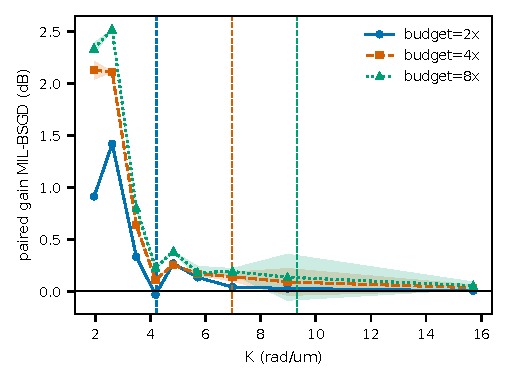
\includegraphics[width=0.95\linewidth]{../code/figures/paper/F4_headline_gain_vs_K.pdf}
\caption{Simulated paired gain (MIL $-$ BSGD) vs.\ spatial frequency $K$,
one curve per contrast budget, 95\% $t$-intervals over three seeds (which
capture initialization sensitivity only). Dashed lines: heuristic
$K_c(B_c)$ [D].}
\label{fig:F4}
\end{figure}

\textbf{Interpretation.} The constrained oracle's own advantage over BSGD
falls with $K$ as MIL's does, which we read as a shrinking achievable
ceiling for any exposure-constrained method rather than a frequency at
which MIL specifically fails. This reading is consistent with the oracle
data but is not a separately tested claim.

Figure~\ref{fig:R1} shows single-seed reconstructions at the three
$K$ points shared by the ablation and robustness studies, $2\times$ budget;
Supplement S1 shows the corresponding exposures and index profiles.

\begin{figure}[htbp]
\centering
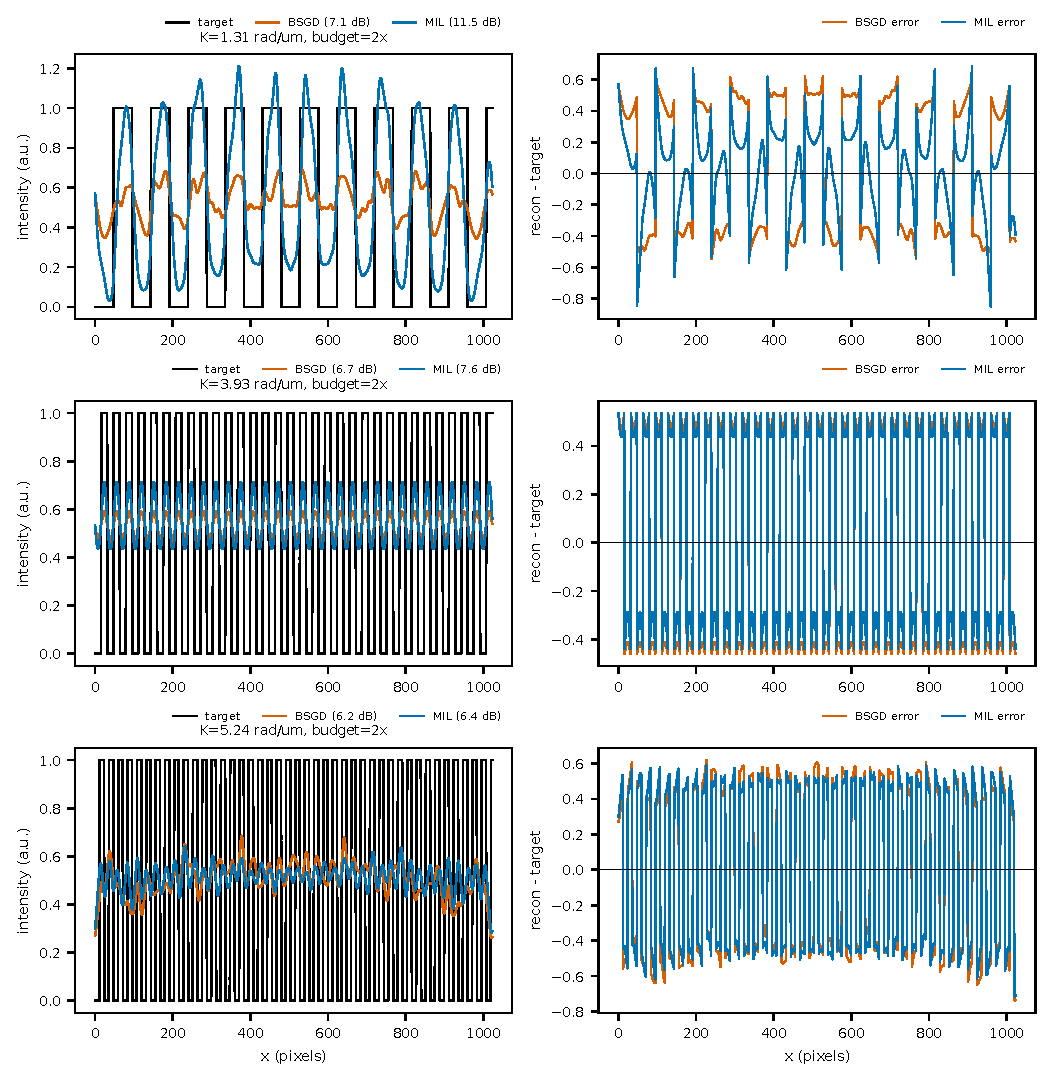
\includegraphics[width=\linewidth]{../code/figures/paper/R1_reconstructions.pdf}
\caption{Target, BSGD and MIL reconstructions (1D intensity profiles, left)
and their errors (right) at $K=\SOneKSub$, \SOneKNear{} and
\SOneKPost\,rad/\textmu m, budget $2\times$, seed \ROneSeedValue.
Illustrative single-seed simulations; Fig.~\ref{fig:F4} carries the
statistics.}
\label{fig:R1}
\end{figure}

\subsection{Failure rate against an oracle reference}
\label{sec:failure-rate}
Because each exposure of a write-once medium consumes material, we also
report how often a method falls far short of what is achievable. An
exposure is counted as failed if its PSNR is more than a threshold below
the constrained oracle's at the same cell; the 2\,dB threshold was fixed
before the results were computed, and 1 and 3\,dB are reported to show
sensitivity to that choice (Table~\ref{tab:failure-rate}). At 2\,dB,
\WastedMediaBSGDFrac\% of BSGD cells and \WastedMediaMILFrac\% of MIL cells
fail; at 3\,dB, \WastedMediaBSGDFracThreeDB\% and
\WastedMediaMILFracThreeDB\%. At 1\,dB the rates are similar
(\WastedMediaBSGDFracOneDB\% and \WastedMediaMILFracOneDB\%): MIL removes
the large shortfalls but not the small ones. These rates are relative to a
numerical reference (ORC), not to a proven optimum, and are computed over
\WastedMediaNConfigs{} grid cells, not over independent physical trials.

\begin{table}[htbp]
\centering
\caption{Simulated failure rate: percentage of the \WastedMediaNConfigs{}
M1 cells in which a method's seed-mean PSNR is more than the column
threshold below the constrained oracle's. GS, LPC, GPC: one deterministic
run per cell; others: mean over three seeds.}
\label{tab:failure-rate}
\begin{tabular}{lccc}
\hline
Method & 1\,dB & 2\,dB & 3\,dB \\
\hline
GS & \WastedMediaGSFracOneDB\% & \WastedMediaGSFrac\% & \WastedMediaGSFracThreeDB\% \\
LPC & \WastedMediaLPCFracOneDB\% & \WastedMediaLPCFrac\% & \WastedMediaLPCFracThreeDB\% \\
GPC & \WastedMediaGPCFracOneDB\% & \WastedMediaGPCFrac\% & \WastedMediaGPCFracThreeDB\% \\
BSGD & \WastedMediaBSGDFracOneDB\% & \WastedMediaBSGDFrac\% & \WastedMediaBSGDFracThreeDB\% \\
RSGD & \WastedMediaRSGDFracOneDB\% & \WastedMediaRSGDFrac\% & \WastedMediaRSGDFracThreeDB\% \\
SAT & \WastedMediaSATFracOneDB\% & \WastedMediaSATFrac\% & \WastedMediaSATFracThreeDB\% \\
MIL & \WastedMediaMILFracOneDB\% & \WastedMediaMILFrac\% & \WastedMediaMILFracThreeDB\% \\
\hline
\end{tabular}
\end{table}

\subsection{Other baselines and the saturation-only surrogate}
\label{sec:baseline-completeness}
Figure~\ref{fig:F4b} compares every non-oracle method with BSGD at
$2\times$. GS (\GSGainMin{} to \GSGainMax\,dB) never improves on BSGD, and LPC
(\LPCGainMin{} to \LPCGainMax\,dB) improves on it by at most
\LPCGainMax\,dB; GPC (\GPCGainMin{} to \GPCGainMax\,dB) differs from LPC by at
most \GPCLPCMaxAbsDiffTwoX\,dB, consistent with both hitting the same
contrast clip. RSGD equals BSGD because its tuned penalty weight is zero.
LPC is the direct closed-form use of the heuristic transfer function, so its
failure to beat BSGD is further evidence that the small-signal picture does
not describe this regime [S].

The saturation-only surrogate asks whether the transport terms are needed at
all. Averaged over $K$, SAT's gain is \SATFracOfMILTwoX\%,
\SATFracOfMILFourX\% and \SATFracOfMILEightX\% of MIL's at
$2\times/4\times/8\times$. Resolved by cell, SAT recovers
\SATFracLowKMin--\SATFracLowKMax\% of MIL's gain at $K=1.96$ and
\SATFracSecondKMin--\SATFracSecondKMax\% at $K=2.62$, but scores below BSGD
in \SATNBelowBSGD{} of the \SATNCells{} cells where the ratio is defined.
The pointwise surrogate is therefore useful only at the lowest spatial
frequencies tested; elsewhere the full recording model is required for any
gain in this benchmark.

\begin{figure}[htbp]
\centering
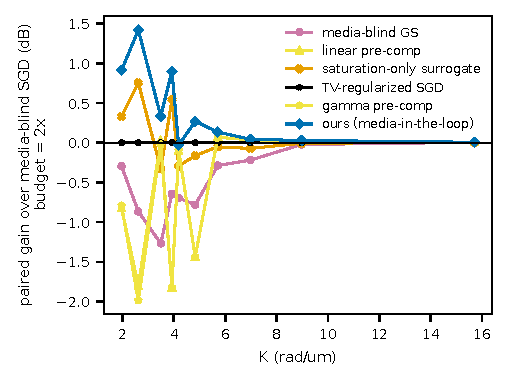
\includegraphics[width=0.8\linewidth]{../code/figures/paper/F4b_baseline_comparison.pdf}
\caption{Simulated paired gain over BSGD for GS, LPC, GPC, RSGD, SAT and
MIL, budget $2\times$. RSGD coincides with BSGD (tuned penalty weight zero).}
\label{fig:F4b}
\end{figure}

\subsection{Compute-matched control}
\label{sec:compute-matched}
MIL's per-iteration cost is about \ComputeMatchRatio$\times$ BSGD's
(measured once, wall-clock). To test whether the gain is an iteration-count
effect, BSGD was rerun with \ComputeMatchRatio$\times$ more iterations at the
three $K$ points of Section~\ref{sec:mechanism}, budget $2\times$
(Supplement S6). With that allowance the paired gain is
\MTwoRGainSub, \MTwoRGainNear{} and \MTwoRGainPost\,dB at
$K=\SOneKSub$, \SOneKNear{} and \SOneKPost\,rad/\textmu m, against
\SOneGBaselineSub, \SOneGBaselineNear{} and \SOneGBaselinePost\,dB when both
arms get the same iteration count (Table~\ref{tab:ablation}, full model). The
extra iterations narrow the gap at the two lower $K$ and leave it unchanged at
$K=\SOneKPost$; it stays positive at all three. Wall-clock is a noisy proxy for compute, so this arm
tests robustness to a much larger baseline iteration budget rather than an
equal-FLOP comparison.

\subsection{Which recording mechanism produces the gain}
\label{sec:mechanism}
\label{sec:s1-ablation}
Table~\ref{tab:ablation} removes one mechanism at a time at three spatial
frequencies, budget $2\times$ (three seeds). Every single-mechanism removal
leaves a positive gain at every $K$; which removal matters depends on $K$.
Linearizing the index map raises the gain at $K=\SOneKSub$ and
\SOneKPost{} but lowers it at \SOneKNear\,rad/\textmu m; removing diffusion
raises it at the two lower $K$. An earlier draft of this paper concluded
that saturation, not transport, is the binding constraint; that conclusion
came from $K$-averaged numbers, and the $K$-resolved data above do not
support it.

\begin{table}[htbp]
\centering
\caption{Simulated paired gain (dB) with one mechanism removed, budget
$2\times$, mean of three seeds. ``No saturation'' replaces the $\tanh$ map
by its linear limit; monomer depletion and dye bleaching still saturate $N$.}
\label{tab:ablation}
\begin{tabular}{lccc}
\hline
Condition & $K=\SOneKSub$ & $K=\SOneKNear$ & $K=\SOneKPost$ \\
\hline
Full model & \SOneGBaselineSub & \SOneGBaselineNear & \SOneGBaselinePost \\
No non-locality ($\sigma=0$) & \SOneGNoNonlocSub & \SOneGNoNonlocNear & \SOneGNoNonlocPost \\
No diffusion ($D_0=0$) & \SOneGNoDiffSub & \SOneGNoDiffNear & \SOneGNoDiffPost \\
No dye depletion & \SOneGNoDyeSub & \SOneGNoDyeNear & \SOneGNoDyePost \\
No saturation ($\tanh$ linearized) & \SOneGNoSatSub & \SOneGNoSatNear & \SOneGNoSatPost \\
\hline
\end{tabular}
\end{table}

\textbf{Mechanism factorial.} Because three mechanisms saturate the dose
response, removing any one leaves the others. We therefore ran all $2^3$
on/off combinations of monomer depletion (removed by holding $u=1$, an
infinite monomer reservoir), dye bleaching ($k_{\text{bleach}}=0$) and the
$\tanh$ map (Supplement S2, Fig.~S2). Removing monomer depletion at fixed
$\kappa$ moves the medium far from its operating point (at unit dose the
cured polymer rises from $N\approx1$ to $N\approx8.7$), so each such cell is
also run with $\kappa$ rescaled to restore $N(E{=}1)=1$ [D]. A final
control removes all three and sets $\kappa=1/(1.5\,t_{\text{total}})$, which
makes the recording exactly BSGD's own linear model up to non-local blur and
shrinkage [D]. In that control the paired gain is \SXGLinearMatchedSub,
\SXGLinearMatchedNear{} and \SXGLinearMatchedPost\,dB; with only the $\tanh$
map active (operating point matched) it is \SXGOnlyTanhMatchedSub,
\SXGOnlyTanhMatchedNear{} and \SXGOnlyTanhMatchedPost\,dB; with only monomer
depletion, \SXGOnlyMonomerSub, \SXGOnlyMonomerNear{} and
\SXGOnlyMonomerPost\,dB; with only dye bleaching (matched),
\SXGOnlyDyeMatchedSub, \SXGOnlyDyeMatchedNear{} and
\SXGOnlyDyeMatchedPost\,dB, at $K=\SOneKSub$, \SOneKNear{} and
\SOneKPost\,rad/\textmu m (with both nonlinearities besides the $\tanh$
map removed, the default $\kappa$ already cures the medium to $N\approx1$ at
unit dose, so the monomer-only cell needs no rescaling). With the
$\tanh$ map and dye bleaching active and monomer depletion removed (matched),
the gain is \SXGNoMonomerMatchedSub, \SXGNoMonomerMatchedNear{} and
\SXGNoMonomerMatchedPost\,dB. The factorial jobs ran on CPU; the full-model
cell reproduces the GPU result of Table~\ref{tab:ablation} to within
\SXDeviceMaxDiff\,dB.

Three observations follow directly from these numbers [S]. First, when the
recording is exactly the media-blind model up to blur and shrinkage, MIL
gains essentially nothing at the two lower $K$, so the gain there requires a
nonlinear dose response; at $K=\SOneKPost$ the linear control's gain
(\SXGLinearMatchedPost\,dB) is comparable to the full model's
(\SOneGBaselinePost\,dB), so the small gain at that $K$ may come from the blur
and shrinkage BSGD ignores rather than from nonlinearity. Second, each of the three saturating mechanisms on
its own, at a matched operating point, produces a gain at the two lower $K$,
so no single mechanism is necessary. Third, among the operating-point-matched
conditions, monomer depletion alone produces the largest gain at every $K$ --
larger than the full model, especially at
$K=\SOneKPost$ -- so combining mechanisms does not add their effects.
Without operating-point matching, removing monomer depletion either saturates
the $\tanh$ map everywhere (both methods then fail equally) or, with the map
linearized, leaves an index modulation an order of magnitude or more
deeper than BSGD assumes, where the gain measures modulation-depth mismatch rather than
saturation (Supplement S2).

\textbf{Interpretation.} In this model the low-$K$ gain comes from designing
through whichever dose-response nonlinearity is present, not from one
privileged mechanism. The matched-operating-point criterion ($N(E{=}1)=1$) is our
choice; other normalizations could change the ranking of the single
mechanisms, though not the null result of the linear control.

\subsection{Dependence on grating slant}
\label{sec:slant}
Holding everything else fixed, the paired gain depends strongly on fringe
slant $\phi$ (Fig.~\ref{fig:F11}, Supplement S3). At $K=1.96$\,rad/\textmu m
it is \SEightGainKLowSlantZero, \SEightGainKLowSlantTwoFive,
\SEightGainKLowSlantFive, \SEightGainKLowSlantTen{} and
\SEightGainKLowSlantTwenty\,dB at $\phi=0^\circ$, $2.5^\circ$, $5^\circ$,
$10^\circ$ and $20^\circ$; at $K=3.93$\,rad/\textmu m,
\SEightGainKMidSlantZero, \SEightGainKMidSlantTwoFive,
\SEightGainKMidSlantFive, \SEightGainKMidSlantTen{} and
\SEightGainKMidSlantTwenty\,dB. The dependence is non-monotone: small slants
increase the gain, and by $10^\circ$ it is below 0.2\,dB. The scalar readout
disagrees with RCWA for slanted gratings (Section~\ref{sec:discussion}), so
the slanted values are model-dependent. The headline results are restricted
to unslanted gratings for that reason, and they should not be read as
predictions for slanted reflection or transmission holograms.

\begin{figure}[htbp]
\centering
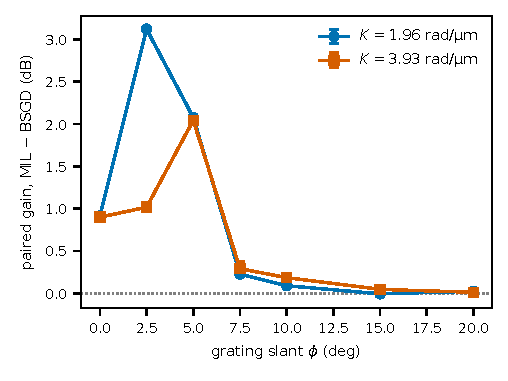
\includegraphics[width=0.7\linewidth]{../code/figures/paper/F11_slant_dependence.pdf}
\caption{Simulated paired gain vs.\ grating slant at two spatial frequencies,
budget $2\times$, 95\% $t$-intervals over three seeds. Slanted values rely on
a scalar readout outside its RCWA-checked range.}
\label{fig:F11}
\end{figure}

\subsection{Robustness to twin miscalibration}
\label{sec:mismatch}
Here the exposure is designed once on the nominal twin and scored, without
re-optimization, on a twin with one parameter perturbed. BSGD uses no
medium parameters in design, so only MIL can be hurt by the error. At the
three $K$ points, budget $2\times$, with $D_0$, $\sigma$, $\kappa$ or
$\Delta n_{\max}$ perturbed by $\pm10$, $\pm25$ or $\pm50\%$, the
$K$-averaged gain ranges from \SThreeWorstWithinFifty{} to
\SThreeBestWithinFifty\,dB (nominal \SThreeNominalGain\,dB; Supplement S4).
$\Delta n_{\max}$ was swept further because our own Bayfol fits with $k_{\text{bleach}}$ held
disagree on it by \BayfolDnMaxRatio$\times$ (Section~\ref{sec:twin-validation-ref}):
the gain is \SThreeDnMaxAtMinusFifty\,dB at $-50\%$,
\SThreeDnMaxAtMostNegative\,dB at $\SThreeDnMaxMostNegativePct\%$,
\SThreeDnMaxAtPlusFifty\,dB at $+50\%$, \SThreeDnMaxAtHundred\,dB at
$+100\%$ and \SThreeDnMaxAtMostPositive\,dB at
$+\SThreeDnMaxMostPositivePct\%$. A twin that underestimates the medium's
index budget by a factor of several can therefore make MIL worse than the
media-blind baseline; between $+100\%$ and $+\SThreeDnMaxMostPositivePct\%$
the sign-change point was not resolved.

\subsection{Joint miscalibration, depth absorption, targets and noise}
\label{sec:joint-mismatch}
With all four parameters drawn independently from
Uniform($\pm$\SSixPctRange\%) in each of \SSixNDraws{} Monte Carlo draws,
reusing the same designed exposures, the $K$-averaged gain ranges from
\SSixWorstDrawGain{} to \SSixBestDrawGain\,dB (mean \SSixMeanGain\,dB,
bootstrap 95\% interval [\SSixBootCILo, \SSixBootCIHi]); \SSixNNegative{} of
\SSixNDraws{} draws are negative. Thirty draws bound the probability of a
negative draw only loosely; this is not a proof that none exists.

Recording with Beer--Lambert attenuation through depth (16 independently
recorded depth slices, same designed exposures) gives \SSevenGainODZero,
\SSevenGainODOneTenth{} and \SSevenGainODThreeTenths\,dB at optical density
0, 0.1 and 0.3. At a single near-cliff point, the gain for three target
families is \SFourGainBarsTwoX{} (bars), \SFourGainSpotsTwoX{} (sparse
spots) and \SFourGainRandomBinaryTwoX\,dB (random binary) at $2\times$, and
a Gaussian detector-noise model at \SFiveNoiseStdPct\% of peak changes it
from \SFiveNoiselessGain{} to \SFiveNoisyGain\,dB (Supplement S8).

% ======================================================================
\section{Twin validation against published data}
\label{sec:twin-validation-ref}
We fit the twin to digitized $\Delta n_1$(dose) curves from Bruder et
al.~\cite{bruder2017bayfol} (Bayfol HX, $K=8.98$\,rad/\textmu m; the
source's own kinetic simulation at 16.7\,mW/cm$^2$ and its measurement at
19.2\,mW/cm$^2$) [L], and a $\Delta n_1$(time) curve from Hsieh et
al.~\cite{hsieh2022pqpmma} (PQ/PMMA, $K=24.94$\,rad/\textmu m, itself a
model output, outside our tested $K$ range) [L]. The curves were read
visually from the published figures (estimated $\pm10\%$ in $x$, $\pm3$--5\%
in $y$), not with a calibrated digitizer.

\textbf{In-sample fits [S].} With $(\kappa,\Delta n_{\max})$ free and
$k_{\text{bleach}}=0.2$ held, best-of-ten fits reach NRMSE
\NRMSEBestInRegime--\NRMSEWorstInRegime{} on the two Bayfol series and
reproduce their rise-then-decline shape (Fig.~\ref{fig:F2}). An earlier fit
with $D_0$ free was poor (NRMSE 0.68--0.87) because the medium configuration
had imported $\Delta n_{\max}$ from a separate dye-screening experiment in
the same source rather than from the dose-response condition being fitted;
with $\Delta n_{\max}$ free that error is removed. The two Bayfol series'
fitted $\Delta n_{\max}$ differ by \BayfolDnMaxRatio$\times$, which a single
material ceiling should not do. With $k_{\text{bleach}}$ also free, in-sample
NRMSE is \HoldoutBSimIn{} (simulated series) and \HoldoutBExpIn{}
(measured series).

\textbf{Held-out prediction [S].} Both Bayfol series are plotted against dose
and the twin is dose-reciprocal at $\gamma=1$, so parameters fitted to one
series predict the other without refitting. With $k_{\text{bleach}}$ held,
fitting the simulated series and predicting the measured one gives NRMSE
\HoldoutASimOut; the reverse gives \HoldoutAExpOut. With $k_{\text{bleach}}$
free the held-out NRMSEs are \HoldoutBSimOut{} and \HoldoutBExpOut. Freeing
$k_{\text{bleach}}$ also changes the fitted parameters: $k_{\text{bleach}}$
comes out at \HoldoutBSimKbleach{} and \HoldoutBExpKbleach{} (below the
default 0.2), and the two series' fitted $\Delta n_{\max}$ become
\HoldoutBSimDnMax{} and \HoldoutBExpDnMax, much closer than the
\HoldoutASimDnMax{} and \HoldoutAExpDnMax{} obtained with $k_{\text{bleach}}$
held. Most of the \BayfolDnMaxRatio$\times$ disagreement noted above is
therefore an artefact of the held dye-bleaching rate. This is a
weak test -- the two series share the material, grating and nearly the same
intensity, and one is itself a model output -- and it does not test transfer
across $K$ or across media.

\begin{figure}[htbp]
\centering
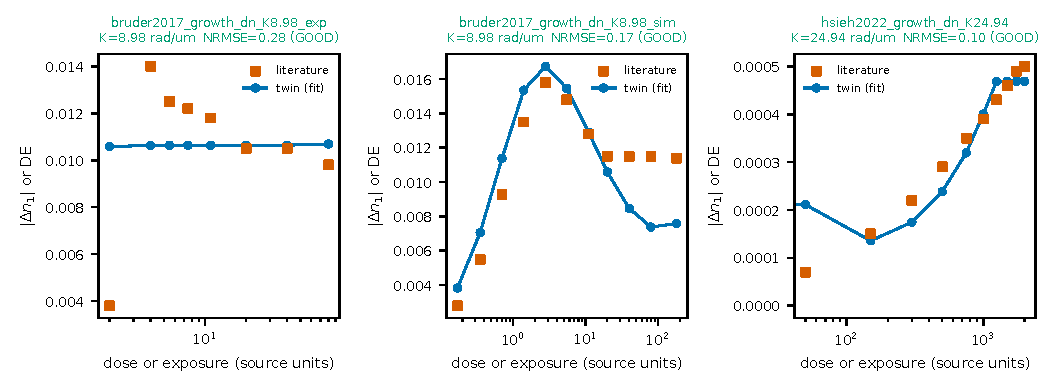
\includegraphics[width=\linewidth]{../code/figures/paper/F2_twin_validation.pdf}
\caption{Twin fits (free $\kappa$, $\Delta n_{\max}$) to digitized literature
curves, best of ten random starts. Left, center: Bayfol HX simulated and
measured series~\cite{bruder2017bayfol}; right: PQ/PMMA~\cite{hsieh2022pqpmma},
outside the tested $K$ range and still rising, so under-constrained.}
\label{fig:F2}
\end{figure}

\textbf{What this establishes.} The twin can reproduce the qualitative
Bayfol dose response with effective parameters; it is not pinned to a real
medium. With $k_{\text{bleach}}=0.2$ held, the dye is almost fully depleted
early in the digitized dose range, so the late decline of $\Delta n_1$ is
produced in the model by diffusive smoothing after polymerization has
stopped; we have not validated that mechanism independently. $D_0$ and
$\sigma$ are identifiable only from multi-$K$ growth-curve families, which
for NPDD media are in subscription-only sources we could not access. The
headline claims rest on the paired design and on the one-sided
miscalibration tests, not on absolute agreement with a real medium.

% ======================================================================
\section{Discussion and limitations}
\label{sec:discussion}
\textbf{Scope.} All results are simulation outputs of one model family,
for one-dimensional transverse recording of binary bar targets, unslanted
gratings, one default medium and three seeds per cell. Whether any of the
gains transfer to a physical photopolymer is untested; the decisive
experiment -- recording optimized and media-blind exposures in a
characterized medium and comparing measured reconstructions -- is future
work.

\textbf{Readout validity.} Against RCWA~\cite{moharam1981rigorous}
(computed with TORCWA~\cite{kim2023torcwa}) over a \RCWAVGridNCases-case grid
of $K$, $\Delta n$, polarization and slant, Kogelnik theory deviates by at
most \RCWAUnslantedMaxDev{} in diffraction efficiency for unslanted
geometries but up to \RCWAVGridMaxDev{} for a $20^\circ$ slant (Supplement
S5) [S]. This check concerns the closed-form reference, and the scalar BPM
used in the design loop shares the paraxial-scalar approximation, so we
restrict validated claims to unslanted gratings. The slant study
(Section~\ref{sec:slant}) shows that this restriction is not a detail: the
simulated gain changes by an order of magnitude over $0$--$10^\circ$.

\textbf{Model simplifications [P].} The recorded profile is uniform through
depth except in the Beer--Lambert check; diffusion uses a spatially averaged
coefficient; the index map and its shape constant are modelling choices;
shrinkage is a placeholder value; the medium parameters are illustrative.
The one-at-a-time ablation measures the effect of removing each mechanism in
the presence of the others; the factorial of Section~\ref{sec:mechanism}
covers interactions among the three saturating mechanisms only. How the
gain varies with the medium itself was checked at one point only
($K=\SOneKPost$\,rad/\textmu m, budget $2\times$): with both arms
re-optimized on media whose $D_0$, $\sigma$ or $\kappa$ is changed by up to
$\pm50\%$, the gain ranges from \STwoGainMin{} to \STwoGainMax\,dB
(nominal \STwoBaselineGain\,dB) [S].

\textbf{Statistics.} Three seeds per cell measure initialization sensitivity,
which is small here; the uncertainty that matters for application --
model and parameter error -- is probed only by the miscalibration studies,
over the ranges stated. The main grid samples \MOneNK{} spatial frequencies;
features between grid points (such as the zero crossing at $2\times$) are
not resolved.

\textbf{Interpretation for practice.} If the twin's qualitative response
is right, the results suggest that exposure-domain optimization through a
recording model is most useful at low spatial frequency and unslanted
geometry, and that its main practical benefit is removing large shortfalls
(Table~\ref{tab:failure-rate}) rather than improving average quality. That
is our reading of the simulated evidence, not a demonstrated property of a
physical system.

\textbf{Calibrating the twin for a new medium.} From our fitting experience
(Supplement S7): $\kappa$ and $\Delta n_{\max}$ are identifiable from a single
dose-response curve; $D_0$ and $\sigma$ need several spatial frequencies;
$\Delta n_{\max}$ must come from the same experimental condition as the curve
being fitted; and the miscalibration study shows that underestimating
$\Delta n_{\max}$ by a large factor is the error most likely to reverse the
benefit.

\begin{backmatter}

\bmsection{Funding}
This work received no external funding. All computation was performed on
the author's personal hardware (a laptop with an NVIDIA RTX 3050 GPU; the
mechanism factorial, reduced compute-matched arm and parameter-sensitivity
jobs ran on its CPU).

\bmsection{Disclosures}
The author declares no conflicts of interest.

\bmsection{Data availability}
{\sloppy
All source code, experiment manifests, raw per-job result files, and the
scripts that generate every number and figure in this paper are available
at \url{https://github.com/ultramagnus23/HoloForge} under
\texttt{part2/code/} (Apache 2.0); \texttt{part2/code/REPRODUCE.md} lists
the commands.
\par}
% The Zenodo DOI below referred to an earlier release (v1.0.0). Mint a new
% versioned release for this revision and update the DOI before submission.
An archived snapshot of an earlier release is at
\url{https://doi.org/10.5281/zenodo.22202762}; the snapshot corresponding to
this version will be archived at submission.

\end{backmatter}

\bibliography{refs}

\end{document}
